% !TeX root = ../index.tex
\section{Peer-to-Peer Networking}
Peer-to-peer networking, P2P in short, means that two or more devices communicate with each other with both serving as a client and a server simultaneously. P2P networks vary in scope a lot. Some networks are global, while some are as small as a couple of devices in a local area network, which is the case in printer sharing and some IoT installations. P2P networks can be standalone or rely on some existing infrastructure, like the internet. The P2P networks that rely on preexisting infrastructure are called overlay networks.

While overlay networks' addressing and routing is usually based on TCP/IP or UDP/IP, they must introduce a separate routing scheme, like a DHT, that works as an index for peers on the network. Since IP only focuses on addressing the computers and not the applications or resources they offer, it can't function as a peer discovery scheme by itself.

Overlay P2P networks must somehow signal the initial peers, also called bootstrap or introductory peers, to connect to at first. This can be done either by including the bootstrap peers' IP addresses in the application code itself or by providing the same information on a regular web page. The bootstrap peers can be also signaled by word-of-mouth between a group of people, or with wireless broadcast, which I will touch a bit on the next section. This said, usually every peer can function as a bootstrap peer, so knowing the connection info of a single peer on the network can potentially introduce you into the network at large.

A simple way to create a P2P network would be to share a single file with anyone who connects to you that has all the IP addresses you've ever connected with. This would be an example of an unstructured P2P network, which could work relatively well in a closed setting, like inside a LAN if there's no support for multicast DNS, or mDNS in short.

\begin{figure}
	
\includegraphics[width=\textwidth]{pictures/unstructured.png}
	\caption{Example topography of an unstructured overlay network}
	\label{Unstructured Overlay Network}
\end{figure}

In contrast to unstructured networks, where peers are connected to at random, structured networks have some logic that is used to form a structured overlay network rather than just connecting to peers as they come.

\begin{figure}
	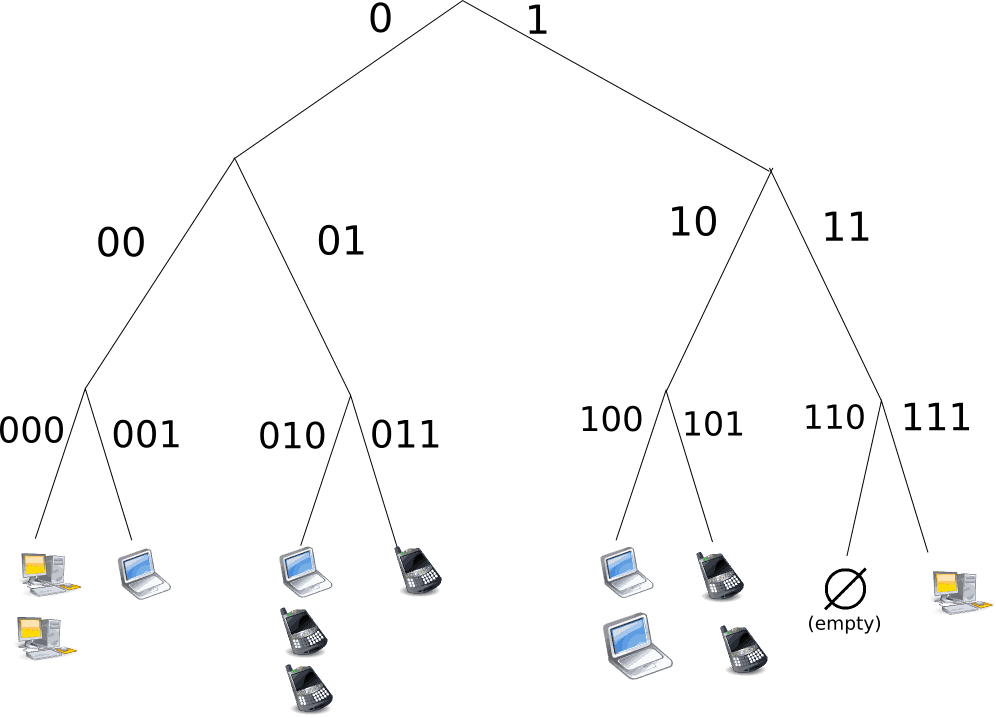
\includegraphics[width=\textwidth]{pictures/structured.png}
	\caption{Example topography of a structured overlay network}
	\label{Structured Overlay Network}
\end{figure}

%TODO: Move the next two sections under P2P?
\section{Role of Latency in Distributed Systems}
It's hardly a surprise, but latency is a huge factor in distributed systems, especially trustless, decentralized ones. Latency is first constrained by the speed of light, and then by hardware and software along the way. In 2012, the global average round-trip delay time to Google's servers was around 100ms.~\cite{Grigorik_undated-mc}
% TODO: Tie this in in some way

In the new space age the maximum possible latency grows very fast, as there could be peers joining to a distributed network from other planets, space ships or stations. This might seem unnecessary to think about in the distributed P2P context for now, but before all that, we have global satellite mesh internet providers, like Starlink. Elon Musk, the founder of SpaceX, which deploys the Starlink network of satellites, claims that there's going to be a round-trip\footnote{Including the user's initial request and received response} latency of about 20 milliseconds between a single satellite and the user.~\cite{Tung_undated-ny} In legacy satellite internet access, the round-trip time even in perfect conditions is about 550 milliseconds.~\cite{noauthor_undated-zc} This difference between legacy and newer satellite internet comes from the difference in their orbits and the sheer amount of satellites involved. Legacy satellite internet uses geostationary orbits, which are very high, beaming on a single face of the earth at a time with limited bandwidth. Newer systems, like Starlink, use a low-earth-orbit, which requires more satellites, since they zoom by at such a speed that constantly changing which satellite you're connected to is a must. The low orbit also means less distance between the satellites and the user. The 20 millisecond latency claimed by Starlink at first seems like a stretch, but is believable when you take into account that inter-satellite links are done by laser, and light can travel about 31 percent faster in a vacuum than in fiber optics.~\cite{Finley2013-wt} Intercontinental latencies can become much lower because of this.

In blockchains, latency plays a role in the efficiency of the power used to achieve consensus. Miners waste energy on a previous block as long as they don't receive information on the winner of the previous block race. It's a waste to drag behind the latest block in terms of information. Simulations by Wei Bi, Huawei Yang, and Maolin Zheng in their paper An Accellerated Method for Message Propagation in Blockchain Networks have shown that if you calculate the round-trip time between the peers that are connected to each other and dropping the ones with larger latencies in favor of lower ones, you can achieve 50\% improvement in average latency with 1 to 2 peers connected. When connectedness grows from the degree of just 1-2 peers up to 20 connected peers, the average latency improvements achieved drop to about 20\%.~\cite{Bi_undated-is} You can't keep multiplexing connections\footnote{Having multiple concurrent stateful connections.} forever, though, and there's a Goldilocks zone for the most effective amount of connections. When connectedness increases, there's shorter routes simply by chance to peers you're not directly connected to, and protocols like publish-subscribe schemes work faster, propagating their messages to the whole network more reliably because there's less relaying happening. There are hardware and software related limitations to the amount of peers. On IPFS, for example, the protocol has been breaking user's routers~\cite{Whyrusleeping2016-ej} because of the high number of incoming connections that need to be routed through NAT\footnote{Network address translation. Hides the local area network from the internet under a different subnet address.}.

Network hops in P2P systems are introduced when two peers are not directly connected to each other, but rather through one or many relays. There are network hops that cannot be easily avoided, like the hops between network routers in the internet. Most of the P2P routing protocols used today are oblivious to the problem of introducing large hops to communications between two peers, trading network performance for network robustness and decentralization. Some DHT-based protocols, like Kademlia, make the assumption that their users have fast internet access, and minimize the average latency by selecting connected peers basically at random.

While the randomness is great for preventing eclipse attacks, they can introduce unnecessary geographical hops between two peers. If two peers are in the same WAN, for example, in Kademlia they might still connect to each other through a network hop going through another continent. This makes routing data between peers inefficient, resulting in preventable lag when sending or receiving data to peers you are not directly connected to.
Now, if we were to rely on IP address geolocation, we could more efficiently connect to peers that are close-by. This is unfortunately impossible in privacy-oriented P2P networks, like mixnets, which aim to hide as much of the packet routing information as possible, by routing individual packets through different peers and hiding IP addresses of two connected peers from each other.~\cite{Harry_Halpin_undated-sq} Obviously, this also has implications on routing and thus Proof of Latency. Optimizing for privacy makes it difficult, if not impossible, to measure and advertise latencies between peers reliably and correctly while obfuscating packet routes.

\subsection{Ad Hoc and Zero Configuration Networking}
Multicast DNS was proposed by Apple in 2013~\cite{Cheshire2013-ja} as a way of discovering peers in a local area network in a zero-configuration manner. It is used today for resource sharing, such as sharing printers. Multicast DNS does not work outside local area networks, since it works by associating names with IP addresses like regular DNS does. The problem is that these names are not quaranteed to be unique, and therefore can be spoofed. If there are two clients with the same name, the first one to respond with its IP address to a query wins.~\cite{Pdp2008-tg} The security of zero-configuration and ad hoc networking must relay on cryptographic identities, so that a peer can verify itself with public-key cryptography, that makes the peers on the network practically unique and thus hard to spoof.

Zero-configuration networking in an unconstrained, global setting is possible with radios, using either dedicated meshnet radios like GoTenna~\cite{GoTenna_undated-km} or Helium~\cite{Helium_undated-jv}, or by using the antennas inside mobile devices to form a network. These types of networks are usually called meshnets or ad hoc networks. Basically, Walkie-Talkies are the simplest form of a P2P network. Problems can arise due to geography blocking signals, or when you want to cross large distances with the transmitting capability of a pocket device. Mesh networking has been used most famously in protests worldwide by using a smartphone app called Firechat.~\cite{Milian2014-mt}

Ad hoc mesh networks have a natural metric for latency, signal strength. They can rely on Bluetooth RSSI\footnote{Received Signal Strength Indication}, or triangulate distances by cooperating with multiple peers. These methods are used to locate emergency calls, and in contact tracing.~\cite{Biddle2020-kl} Mesh networks, while being peer to peer and not relying on existing infrastructure like overlay networks, still need routing and multiple hops if one wants to reach peers that are not in the operating range of the communication method used. Even ad hoc networks could benefit from having a Proof of Latency, although the proofs should be updated way more frequently because of their mobile nature.

\subsection{Distributed Hash Tables}
Distributed hash tables are a way of pointing content to peers in a distributed network. In addition to indexing content in content-addressed networks like IPFS~\cite{Labs_undated-uw}, they can function as routing tables, and have been developed to remove bottlenecks in peer search. A hash table is a key-value mapping from a to b. What makes them distributed is the fact that the data stored is meant to be distributed between peers, with not a single peer keeping all the available data in its hash table, but relaying queries for resources it does not have to other peers on the network. There are multiple versions of DHTs with different methods for prioritizing certain peers, using tree structures, sorting by identifiers, using computational trust et cetera.

In addition to identifier closeness, DHTs can force a certain network behavior by peer scoring and constructing a web of trust. For example, a peer could only advertise peers that have been connected over a period of time, or enforce reconnecting to disconnected peers that have a good reputation. Computational trust is bayesian in nature, optimizing a single value over time, and simulating remembrance and forgettance. A widely used trust system like this is TrustGuard, implemented in the blockchain framework Tendermint.~\cite{Srivatsa2005-ib, Jeff_Foley2018-zt}

Most of the DHT algorithms were invented in the early 2000s, with Kademlia being one of them. DHTs mostly differ just by how distance is defined, and how the neighbors are chosen.~\cite{Cai2015-ra}

\subsubsection{Kademlia}
Kademlia is a DHT designed by Petar Maymounkov and David Mazières in 2002. It is based on a tree of identifiers which are split across peers on a network. The identifiers are 160 bits, e.g. a SHA-1 hash of some larger data. Kademlia tries to improve upon previous DHT-based routing algorithms by introducing a symmetric XOR metric for distance between node IDs in the key space.~\cite{Petar_Maymounkov2020-sx} These IDs are sorted in a binary search tree, with each node's position determined by the shortest unique prefix of its ID, like shown in diagram \ref{Structured Overlay Network} on page \pageref{Structured Overlay Network}. Kademlia makes sure that any node in the network can locate any other node by its ID by making sure that each node knows at least one of the nodes in each subtree.

A single query in Kademlia has been shown in real-world tests to result in an average of 3 network hops, meaning that the query gets relayed through two peers before reaching the requested resource.~\cite{Roos2013-mb} Network hops are a necessary evil in distributed systems, and Kademlia does well in requiring on average a log(n) queries in a network of n nodes. Since the closeness metric is based on a similarity search rather than a measurement, the closest peer is only closest by the identifier, not by network latency.~\cite{Eigenmann2020-zm}

The randomness of Kademlia is great at averaging the network hops required to reach a scarce resource. While this is great for network security, the downside is that it also averages latency, reducing overall performance of the network.

Kademlia protocol has four remote procedure calls, or RPCs in short. These are PING, STORE, FIND\_NODE, and FIND\_VALUE. A Kademlia participant's most important operation is node lookup, which is locating k closest nodes to a given node ID. It is a recursive operation, which starts by picking alpha closest nodes from its closest non-empty bucket, and sending them all FIND\_NODE calls. This is repeated until the initiator has queried and got responses from all k closest nodes it has seen.

\subsection{Eclipse Attacks}
Although Kademlia is most widely used with random hashed identifiers, the distance metric stays the same. By forging identities that are close-by, you can advertise false friends which take over the search space. For example, in a 2019 paper "Eclipsing Ethereum Peers with False Friends" by S. Henningsen, D. Teunis, M. Florian, and B. Scheuermann, they demonstrate that to eclipse a victim in Ethereum P2P network, you need to fill its 8 slots for outbound connections, and fill 17 slots for inbound connections to completely deny service without going through the attacker's nodes.~\cite{Henningsen2019-mf}

Less structured, random ways of forming connections in an overlay network, like Kademlia, protect against eclipse attacks quite well because of the high connectivity and low locality. Introducing peer scoring and making the network topology more structured opens up possibilities for an attacker to game the scoring system, making sure the target connects to lots of sybil peers eclipsing it. Thus, protecting against eclipse attacks is a balancing act that requires an overlay network to retain some elements of an unstructured network while improving general performance with a structured group of peers.~\cite{Mao2020-ee} This balancing act is seen as a multi-armed bandit problem of exploration and exploitation in the 2020 paper "Perigee: Efficient Peer-to-Peer Network Design for Blockchains" by Y. Mao, S. Deb, S.B. Venkatakrishnan, S. Kannan, and K. Srinivasan.


\subsection{Sybil Attacks}
Sybil attacks mean creating multiple false identities in a P2P network to achieve a botnet-like effect. This could result in gaining disproportionate influence in decentralized governance, block voting, block producing et cetera. An eclipse attack usually involves a sybil attack to create the peers that are used to eclipse peers with.

% TODO: More stuff here
